 \documentclass[a4paper,11pt]{article}

\usepackage{fancyhdr}
\usepackage[dvips]{graphicx}  % for eps and MatLab Diagrams
\usepackage{amsmath}
\usepackage{psfrag,color}
\usepackage[framed]{/Applications/TeX/mcode}

\pagestyle{fancy}

\begin{document} % Begin Document

% Title
\title{\textsc{Minimal Bounding Shapes in 2 and 3 Dimensions}}

% Authors and Contact Information
\author{\textbf{John R. D'Errico}\\
Email: woodchips@rochester.rr.com}

\maketitle

\section{Introduction - Minimal Bounding Shapes}

This document will discuss the estimation of several basic enclosing shapes around
sets of points in 2 and 3 dimensions.

But first, why would you wish to use these tools at all? A minimal enclosing object of
a well defined basic shape may be of use to roughly characterize objects, perhaps in an 
image. Perhaps one needs simple estimates of an area enclosed, or of the center of a
roughly circular or elliptical object. Some examples might be bacteria, crystals, granular
particles, film grain, etc.

The basic codes I'll discuss are:

\begin{itemize}
  \item Rectangles - \mcode{MINBOUNDRECT}
  \item Circles - \mcode{MINBOUNDCIRCLE}
  \item Spheres (3-d) - \mcode{MINBOUNDSPHERE}
  \item Ellipses - \mcode{MINBOUNDELLIPSE}
  \item Ellipsoids (3-d) - \mcode{MINBOUNDELLIPSOID}
\end{itemize}

One feature that all these codes have in common is the initial use of a convex
hull call. Since all of the shapes we will consider here are convex objects, no point that
is inside the convex hull of the data set need be considered. Removal of those interior
data points will often result in a dramatic reduction in the time required otherwise.

\begin{figure}
\centering
    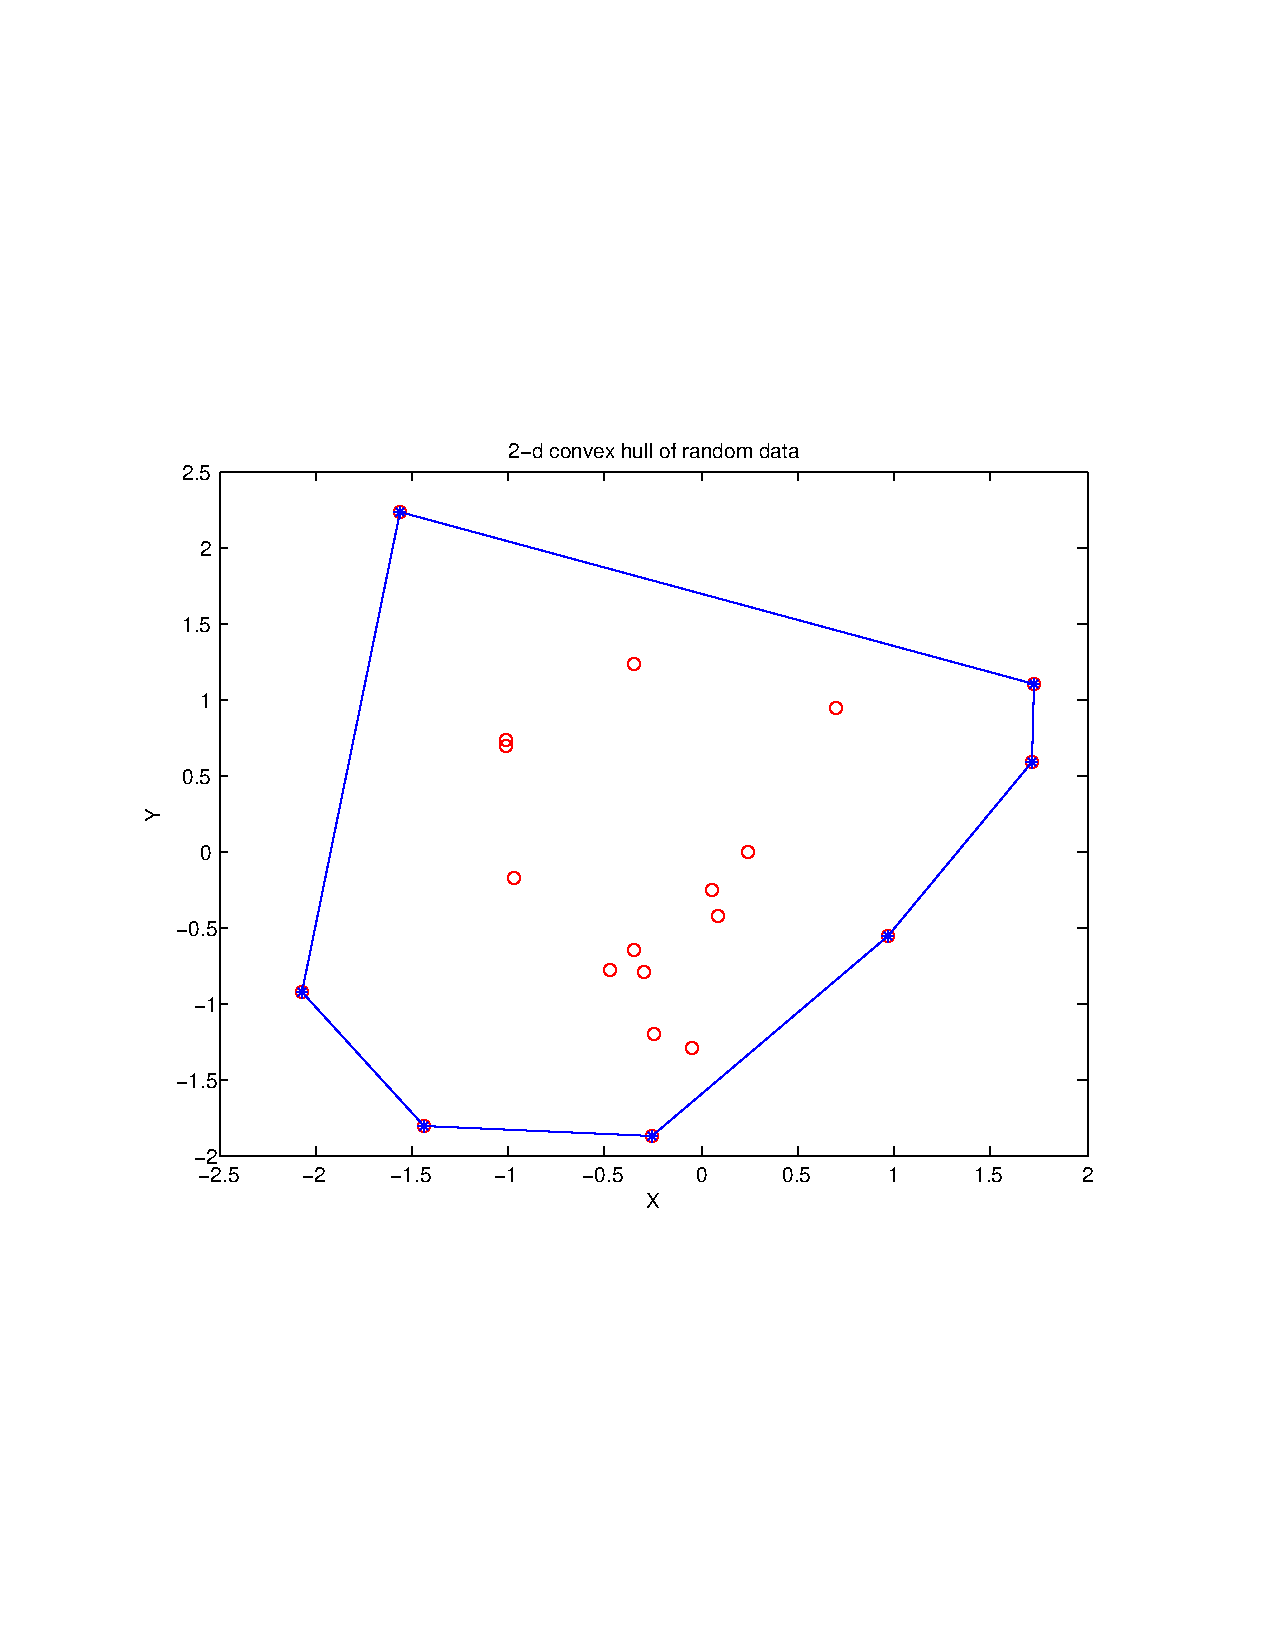
\includegraphics[width=5in]{convhull.pdf}
        \caption{Example of a convex hull in 2-d}
\end{figure}

\bigskip

\section{Minimal Area Rectangles}

Somewhat distinct from the other tools here is rectangle estimation. It is simply done,
especially when you start from the convex hull. If we assume that the minimum bounding
rectangle must have one (or more) edges parallel to one of the edges of the convex hull,
then the task is a simple one indeed. Merely check every edge of the convex hull,
effectively spreading a pair of calipers around the object at that angle. One chooses that
edge which produces the minimum area from all the possible rectangles.

This scheme will generally be a quite efficient one, since most of the time a convex hull 
is composed of relatively few edges. Even in the rare event where every single point
supplied is also found to be a part of the convex hull itself, the rectangle computation is
fast enough to be efficient.

\bigskip


\section{Minimal Radius Circles and Spheres}

Circular regions are slightly more complex than are rectangles, but still simple enough.
Again, we start with all of the points making up the convex hull. Arbitrarily pick any three
of those points. Find the unique minimum radius enclosing circle that contains those three
points. If every other point is inside the above circle, then we are done. Pick that single
point which lies furthest outside of the circle, and find the enclosing circle of this set of
four points. That larger enclosing circle will have either 2 or three of those points on its
circumference. Repeat until no more points lie external to the current enclosing circle.

The basic algorithm above is a simple iterative scheme which will generally terminate
after only a few iterations. One aspect of this that is worth further discussion is the
computation of a circum-circle. Given any three points in the (x,y) plane, $(x_1,y_1)$,
$(x_2,y_2)$, $(x_3,y_3)$, there are two distinct possibilities. Either two of the three
points lie on a diameter
of a circle that also contains the third point, or all three of the points must lie exactly on the
circumference of a circle.

In the latter event, that circle with unknown radius $R$ and center $(\mu_x,\mu_y)$ must
satisfy (1), (2), and (3).

\begin{equation} \tag{1}
   (x_1 - \mu_x)^2 + (y_1 - \mu_y)^2 = R^2
\end{equation}
\begin{equation} \tag{2}
   (x_2 - \mu_x)^2 + (y_2 - \mu_y)^2 = R^2
\end{equation}
\begin{equation} \tag{3}
   (x_3 - \mu_x)^2 + (y_3 - \mu_y)^2 = R^2
\end{equation}

We can eliminate the quadratic terms in the unknowns simply by subtracting pairs of 
those expressions to yield (4) and (5), linear in the unknowns $(\mu_x,\mu_y)$.

\begin{equation} \tag{4}
   2(x_1 - x_2)\mu_x + 2(y_1 - y_2)\mu_y = x_1^2 - x_2^2 + y_1^2 - y_2^2  
\end{equation}
\begin{equation} \tag{5}
   2(x_1 - x_3)\mu_x + 2(y_1 - y_3)\mu_y = x_1^2 - x_3^2 + y_1^2 - y_3^2  
\end{equation}

Solve that linear system of equations for $(\mu_x,\mu_y)$. then use (1) to obtain $R$.

This basic scheme of differencing to drop out the nonlinear terms, then solving a linear
system for the center of the circle will also apply to computation of a circum-sphere in
any number of dimensions.

\bigskip


\bigskip

\section{Minimal Area Enclosing Ellipses and Minimum Volume Enclosing Ellipsoids}

Ellipses and ellipsoids are yet a step higher in complexity than are circles. In a simple form,
the equation (6) of an ellipse with center $(\mu_x,\mu_y)$, has axis lengths of $a_x$ and $a_y$
along the x and y axes respectively. Clearly, if $a_x = a_y$, then the ellipse is circular.

\begin{equation} \tag{6}
(\frac{x-\mu_x}{a_x})^2 + (\frac{y - \mu_y}{a_y})^2 = 1
\end{equation}

Of course, the form in (6) does not allow for any eccentricity. We can allow for an eccentricity
by writing the ellipse as the quadratic form in (7).

\begin{equation} \tag{7}
([x,y] - [\mu_x,\mu_y])
\begin{bmatrix} H_{xx} & H_{xy}  \\ H_{xy} & H_{yy} \end{bmatrix}
([x,y] - [\mu_x,\mu_y])^T = 1
\end{equation}

Enclosing circle parameters (the center of the circle) were derivable from the linear system
{(4), (5)}. That approach will fail here though, since the quadratic terms do not drop out. A
partial solution arises from a technique called partitioned least squares. 





\end{document}

